\startchapter{Hardware Trojans}
\label{chapter:hardwareTrojans}

\newlength{\savedunitlength}
\setlength{\unitlength}{2em}
\section{Background} \label{sec:trojanBackGround}
\acrfull{ICs} are continuously decreasing in size whilst increasing in complexity.
These trends require ever more people and sophisticated means of manufacture which in turn creates security vulnerabilities.
Products developed by semiconductor companies tend to be compromised in one of two ways.
First, due to its complexity it is rare for an \acrshort{IC} to be entirely manufactured within a single company.
Frequently, steps in the production-chain are outsourced.
It is within these 'third-party' contributors that products can be maliciously modified.
Secondly, for various reasons, employees of trusted contributors have been known to make modifications~\cite{trojanSurvey2014}.
\acrshort{IC}s are an integral part of every facet of the modern world.
Proper application of a trojan can provide information, control of mechanical systems, surveillance and more to an unauthorized party.


\section{Topology} \label{sec:topology}
The discussion, detection and evaluation of hardware trojans requires a comprehensive means of description.
Several hardware trojan taxonomies have been proposed~\cite{taxonomy1, taxonomy2, taxonomy3, taxonomy4}.
In~\cite{taxonomy1}, trojans were organized based solely on their activation mechanisms.
A taxonomy based on the location, activation and action of a trojan was presented in \cite{taxonomy2}, \cite{taxonomy3}.
However, these approaches do not consider the manufacturing process.
Another taxonomy was proposed in~\cite{taxonomy4} which employs five categories: insertion, abstraction, activation, effect, and location.
While this is more extensive than previous approaches, it fails to account for the physical characteristics of a trojan.
An additional taxonomy was proposed in~\cite{samerAttribute} which considers all attributes a hardware trojan may posses.
This taxonomy is the most comprehensive and was selected as the means of description for this work.
\begin{figure}
	\centering
	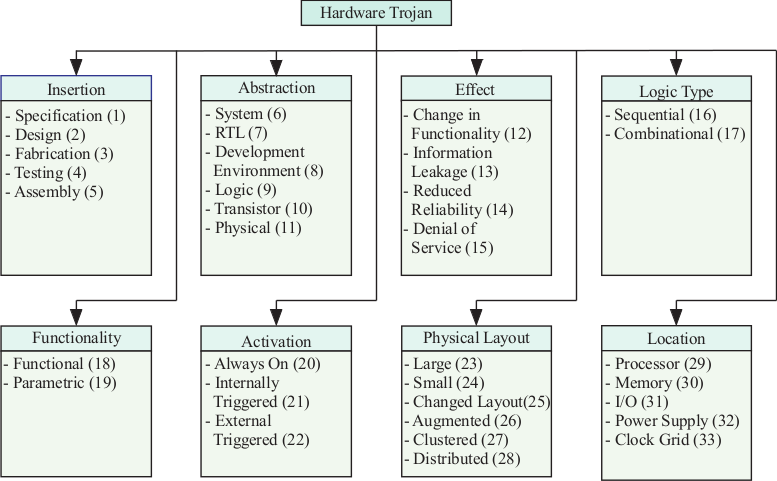
\includegraphics[width=1.0\linewidth]{figures/HW_trojan}
	\caption{The thirty-three attributes of the hardware trojan taxonomy in~\cite{samerAttribute}.}
	\label{fig:HW_trojan}
\end{figure}
It is comprised of thirty-three attributes organized into eight categories as shown in Fig.~\ref{fig:HW_trojan}.
These categories can be arranged into the following four levels as indicated in Fig.~\ref{fig:trojan_life_cycle}.
\begin{enumerate}
	\item The \textbf{insertion} (chip life-cycle) level/category comprises the attributes pertaining to the IC production stages.
	\item The \textbf{abstraction} level/category corresponds to where in the IC abstraction the trojan is introduced.
	\item The \textbf{properties} level comprises the behavior and physical characteristics of the trojan.
	\item The \textbf{location} level/category corresponds to the location of the trojan in the IC.
\end{enumerate}
The properties level consists of the following categories.
\begin{itemize}
	\item The \textbf{effect} describes the disruption or effect a trojan has on the system.
	\item The \textbf{logic type} is the circuit logic that triggers the trojan, either combinational or sequential.
	\item The \textbf{functionality} differentiates between trojans which are functional or parametric.
	\item The \textbf{activation} differentiates between trojans which are always on or triggered.
	\item The \textbf{layout} is based on the physical characteristics of the trojan.
\end{itemize}
\begin{figure}
	\centering
	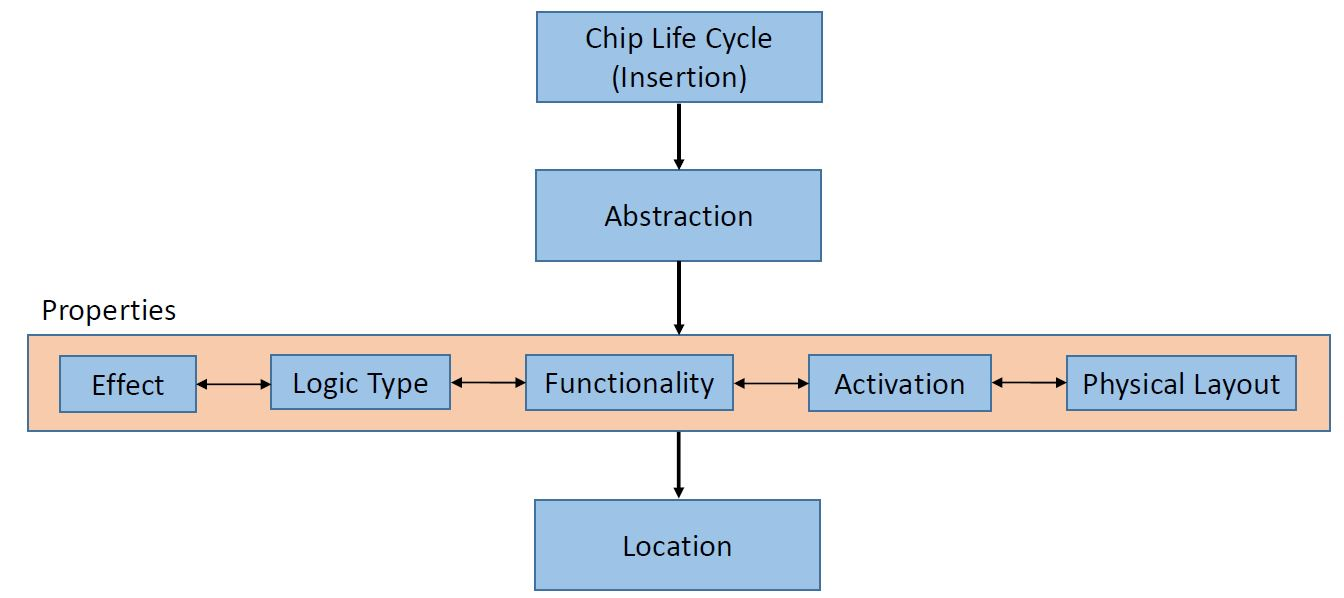
\includegraphics[width=0.8\linewidth]{figures/trojan_life_cycle}
	\caption{The hardware trojan levels \cite{samerAttribute}.}
	\label{fig:trojan_life_cycle}
\end{figure}

\begin{table*}
	\[
	\newcommand\scalemath[2]{\scalebox{#1}{\mbox{\ensuremath{\displaystyle #2}}}}
	\mathbf{R} =
	\left[
	\scalemath{0.5}{
		\begin{array}{l||c|c|c|c|c||c|c|c|c|c|c||c|c|c|c|c|c|c|c|c|c|c|c|c|c|c|c|c||c|c|c|c|c}
		A & 1$~$ & 2$~$  & 3$~$ & 4$~$& 5$~$ & 6$~$  & 7$~$ & 8$~$ & 9$~$ & 10  & 11 & 12& 13 & 14  & 15 & 16& 17 & 18  & 19 & 20& 21 & 22  & 23 & 24& 25 & 26  & 27 & 28 & 29 &30 & 31 & 32 & 33\\ \hline \hline
		1 & 0 & 1 & 0 & 0 & 0 & 1 & 0 & 0 & 0 & 0 & 0 &  &  &  &  &  &  &  &  &  &  &  &  &  &  &  &  &   &  &  &  &  &  \\ \hline
		2 & 0 & 0 & 1 & 0 & 0 & 0 & 1 & 0 & 0 & 0 & 0 &  &  &  &  &  &  &  &  &  &  &  &  &  &  &  &  & &  &  &  &  &   \\ \hline
		3 & 0 & 0 & 0 & 1 & 0 & 0 & 0 & 0 & 0 & 0 & 1 &  &  &  &  &  &  &  &  &  &  &  &  &  &  &  &  & &  &  &  &  &   \\  \hline
		4 & 0 & 0 & 0 & 0 & 1 & 1 & 0 & 0 & 1 & 0 & 0 &  &  &  &  &  &  &  &  &  &  &  &  &  &  &  &  &&  &  &  &  &    \\  \hline
		5 & 0 & 0 & 0 & 0 & 0 & 1 & 0 & 0 & 0 & 0 & 0 &  &  &  &  &  &  &  &  &  &  &  &  &  &  &  &  &  &  &  &  &  &  \\  \hline \hline
		6 &  &  &  &  &  & 0 & 1 & 0 & 0 & 0 & 0 &1 & 1 & 0 & 1 & 0 & 0 & 1 & 1 & 1 & 0 & 0 & 0 & 0 & 0 & 0 & 0 & 0  &  &  &  &  &  \\ \hline
		7 &  &  &  &  &  & 0 & 0 & 1 & 0 & 0 & 0 &1 & 0 & 0 & 1 & 1 & 1 & 1 & 0 & 1 & 1 & 1 & 1 & 1 & 0 & 0 & 0 & 0  &  &  &  &  &   \\ \hline
		8 &  &  &  &  &  & 0 & 0 & 0 & 1 & 0 & 0 &1 & 0 & 0 & 1 & 1 & 1 & 1 & 0 & 1 & 1 & 1 & 1 & 1 & 1 & 1 & 1 & 1  &  &  &  &  &   \\ \hline
		9 &  &  &  &  &  & 0 & 0 & 0 & 0 & 1 & 0 & 1 & 0 & 0 & 1 & 1 & 1 & 1 & 0 & 1 & 1 & 1 & 0 & 0 & 0 & 0 & 0 & 0 &  &  &  &  &    \\ \hline
		10 &  &  &  &  &  & 0 & 0 & 0 & 0 & 0 & 1 & 1 & 0 & 1 & 0 & 0 & 1 & 1 & 1 & 1 & 0 & 0 & 0 & 1 & 0 & 1 & 1 & 0  &  &  &  &  &  \\  \hline
		11 &  &  &  &  &  & 0 & 0 & 0 & 0 & 0 & 0 &1 & 1 & 1 & 0 & 0 & 0 & 1 & 1 & 1 & 0 & 0 & 1 & 1 & 1 & 1 & 1 & 1  &  &  &  &  &    \\  \hline \hline
		12 & &  &  &  &  &  &  &  &  &  &  & 0 & 0 & 0 & 0 & 1 & 1 & 1 & 0 & 1 & 1 & 1 & 1 & 1 & 1 & 1 & 1 & 1&1 & 1 & 1 & 1 & 1 \\ \hline
		13 & &  &  &  &  &  &  &  &  &  &  &0 & 0 & 0 & 0 & 0 & 1 & 0 & 1 & 1 & 0 & 1 & 0 & 1 & 0 & 1 & 1 & 1&1 & 1 & 1 & 1 & 1 \\ \hline
		14 &&  &  &  &  &  &  &  &  &  &  & 0 & 0 & 0 & 0 & 0 & 0 & 0 & 1 & 1 & 0 & 0 & 0 & 1 & 0 & 1 & 1 & 1&1 & 1 & 1 & 1 & 1 \\ \hline
		15 & &  &  &  &  &  &  &  &  &  &  &0 & 0 & 0 & 0 & 1 & 1 & 1 & 0 & 1 & 1 & 1 & 1 & 1 & 1 & 1 & 1 & 1&1 & 0 & 1 & 1 & 1 \\ \hline
		16 & &  &  &  &  &  &  &  &  &  &  &1 & 0 & 0 & 1 & 0 & 0 & 1 & 0 & 0 & 1 & 1 & 1 & 0 & 1 & 1 & 1 & 1&1 & 1 & 1 & 1 & 1 \\ \hline
		17 & &  &  &  &  &  &  &  &  &  &  &1 & 1 & 0 & 1 & 0 &0 & 1 & 0 & 1 & 1 & 1 & 1 & 1 & 1 & 1 & 1 & 1&1 & 1 & 1 & 1 & 1 \\ \hline
		18 & &  &  &  &  &  &  &  &  &  &  &1 & 0 & 0 & 1 & 1 & 1 & 0 & 0 & 1 & 1 & 1 & 1 & 1 & 1 & 1 & 1 & 1&1 & 1 & 1 & 1 & 1 \\ \hline
		19 & &  &  &  &  &  &  &  &  &  &  &0 & 1 & 1 & 0 & 0 & 0 & 0 & 0 & 1 & 0 & 0 & 0 & 1 & 0 & 1 & 0 & 1&0 & 0 & 1 & 1 & 1 \\ \hline
		20 & &  &  &  &  &  &  &  &  &  &  &1 & 1 & 1 & 1 & 0 & 1 & 1 & 1 & 0 & 0 & 0 & 1 & 1 & 1 & 1 & 1 & 1&1 & 1 & 1 & 1 & 1 \\ \hline
		21 & &  &  &  &  &  &  &  &  &  &  &1 & 0 & 0 & 1 & 1 & 1 & 1 & 0 & 0 & 0 & 0 & 1 & 1 & 0 & 1 & 1 & 1&1 & 1 & 1 & 1 & 1 \\ \hline
		22 & &  &  &  &  &  &  &  &  &  &  &1 & 1 & 0 & 1 & 1 & 1 & 1 & 0 & 0 & 0 & 0 & 0 & 1 & 0 & 1 & 1 & 0&1 & 1 & 1 & 1 & 1 \\ \hline
		23 & &  &  &  &  &  &  &  &  &  &  &1 & 0 & 0 & 1 & 1 & 1 & 1 & 0 & 1 & 1 & 0 & 0 & 0 & 1 & 1 & 1 & 1&1 & 1 & 0 & 0 & 0  \\ \hline
		24 & &  &  &  &  &  &  &  &  &  &  &1 & 1 & 1 & 1 & 0 & 1 & 1 & 1 & 1 & 1 & 1 & 0 & 0 & 0 & 1 & 1 & 0&1 & 1 & 1 & 1 & 1 \\ \hline
		25 &&  &  &  &  &  &  &  &  &  &  & 1 & 0 & 0 & 1 & 1 & 1 & 1 & 0 & 1 & 0 & 0 & 1 & 0 & 0 & 1 & 1 & 0& 1 & 1 & 1 & 1 & 1\\ \hline
		26 & &  &  &  &  &  &  &  &  &  &  &1 & 1 & 1 & 1 & 1 & 1 & 1 & 1 & 1 & 1 & 1 & 1 & 1 & 1 & 0 & 1 & 1& 1 & 1 & 1 & 1 & 1\\ \hline
		27 & &  &  &  &  &  &  &  &  &  &  &1 & 1 & 1 & 1 & 1 & 1 & 1 & 0 & 1 & 1 & 1 & 1 & 1 & 1 & 1 & 0 & 0 &1 & 1 & 1 & 1 & 1\\ \hline
		28 & &  &  &  &  &  &  &  &  &  &  &1 & 1 & 1 & 1 & 1 & 1 & 1 & 1 & 1 & 1 & 0 & 1 & 0 & 0 & 1 & 0 &0 &1 & 1 & 1 & 1 & 1\\ \hline \hline
		29 & &  &  &  &  &  &  &  &  &  &  & &  &  & &  &  &  &  &  &  &  &  &  &  &  &  & & &  &  &  & \\ \hline
		30 & &  &  &  &  &  &  &  &  &  &  & &  &  & &  &  &  &  &  &  &  &  &  &  &  &  & & &  &  &  & \\ \hline
		31 & &  &  &  &  &  &  &  &  &  &  & &  &  & &  &  &  &  &  &  &  &  &  &  &  &  & & &  &  &  & \\ \hline
		32 & &  &  &  &  &  &  &  &  &  &  & &  &  & &  &  &  &  &  &  &  &  &  &  &  &  & & &  &  &  & \\ \hline
		33 & &  &  &  &  &  &  &  &  &  &  & &  &  & &  &  &  &  &  &  &  &  &  &  &  &  & & &  &  &  & \\
		\end{array}
	}
	\right ]
	\label{ss1}
	\]
\end{table*}
The relationships between the trojan attributes shown in Fig.~\ref{fig:HW_trojan} can be described using a matrix $\mathbf{R}$~\cite{samerAttribute}.
%Systematic analysis of matrix $\mathbf{R}$ provides useful insight into the overall nature of a subject.
%A procedure used to develop the nature of a subject has been described in~\cite{samerAttribute} and is referred to as Classification.
Entry $r(i,j)$ in $\mathbf{R}$ indicates whether or not attribute $i$ can lead to attribute $j$.
For example, $r(2,3) = 1$ indicates that design (attribute 2) can lead to fabrication (attribute 3).
This implies that if an IC can be compromised during the design phase (attribute 2), it may influence the fabrication phase (attribute 3).

The matrix $\mathbf{R}$ is divided into sub matrices as follows
\[
\newcommand\scalemath[2]{\scalebox{#1}{\mbox{\ensuremath{\displaystyle #2}}}}
\mathbf{R} =\left[
\scalemath{1.1}{
	\begin{array}{l*{3}{c}}
	\mathbf{R_1} ~ & ~ \mathbf{R_{12}} ~ & ~ 0 ~  &  ~ 0   \\
	0         & \mathbf{R_2}      &\mathbf{R_{23}}       & ~ 0 \\
	0          & 0           & \mathbf{R_3}          & ~ \mathbf{R_{34}} \\
	0          & 0           & 0                & ~ \mathbf{R_4} \\
	\end{array}
}
\right]
\label{R}
\]
where $\mathbf{R_1}$, $\mathbf{R_2}$, $\mathbf{R_3}$ and $\mathbf{R_4}$ indicate the attribute relationships within a category.
For example, $\mathbf{R_1}$ is given by
\[
\newcommand\scalemath[2]{\scalebox{#1}{\mbox{\ensuremath{\displaystyle #2}}}}
\mathbf{R_1} =\left[
\scalemath{1.0}{
	\begin{array}{l|*{11}{c}}
	A & 1$~$ & 2$~$  & 3$~$ & 4$~$& 5$~$\\ \hline
	1 & 0 & 1 & 0 & 0 & 0  \\
	2 & 0 & 0 & 1 & 0 & 0  \\
	3 & 0 & 0 & 0 & 1 & 0  \\
	4 & 0 & 0 & 0 & 0 & 1  \\
	5 & 0 & 0 & 0 & 0 & 0  \\
	\end{array}
}
\right ]
\label{R1}
\]
Submatrix $\mathbf{R_{12}}$ relates the attributes of the insertion category to the attributes of the abstraction category.
An example of this submatrix is
\[
\newcommand\scalemath[2]{\scalebox{#1}{\mbox{\ensuremath{\displaystyle #2}}}}
\mathbf{R_{12}} =\left[
\scalemath{1.0}{
	\begin{array}{l|*{11}{c}}
	A & 6$~$  & 7$~$ & 8$~$ & 9$~$ & 10  & 11\\ \hline
	1  & 1 & 0 & 0 & 0 & 0 & 0 \\
	2  & 0 & 1 & 0 & 0 & 0 & 0 \\
	3  & 0 & 0 & 0 & 0 & 0 & 1 \\
	4  & 1 & 0 & 0 & 1 & 0 & 0 \\
	5  & 1 & 0 & 0 & 0 & 0 & 0 \\
	\end{array}
}
\right ]
\label{R12}
\]

%%%%%%%%%%%%%%%%%%%%%%%%%%%%%%%%%%%%%%%%%%%%%%%%%%
\section{Hardware Trojan Analysis Techniques} \label{sec:techniques}
%\color{red}
The benefit of the taxonomy described in section~\ref{sec:topology} is that it comprehensive and structured design provides the ability to develop systematic methods of analysis.
A pair of techniques have already been proposed that provide additional insight.

\subsection{Classification}  \label{sec:techniqueClassification}
An observed hardware trojan must have its descriptive attributes extracted.
These attributes are then used as input to a systematic process of scanning the rows and columns of matrix $\mathbf{R}$; this technique can be used to gain valuable insight into the characteristics of the trojan.
This process is described in detail in~\cite{samerAttribute,samerDissertation}.
The observed attributes can be used to determine the possible locations of a trojan within the design and in which manufacturing phases it can be inserted.
Conversely, the phase a trojan was inserted can be used to determine which abstraction levels are vulnerable,
the trojan properties, and what locations can be compromised.
To easily understand the characteristics of a trojan, a directed graph is generated from $\mathbf{R}$.
Attributes are represented by nodes and their relationships by edges.\newline\newline
Consider a trojan that has the following attributes:
\begin{itemize}
	\item causes denial of service (DoD) (attribute 15),
	\item composed of combinational logic (attribute 17),
	\item functional (attribute 18), and
	\item externally triggered (attribute 22).
\end{itemize}
An examination of $\mathbf{R}$ leads to the graph shown in Fig.~\ref{fig:full2}.
If it is determined that it is not possible to insert the trojan in the design phase (attribute 2), then
attribute 2 can be removed from the graph.
Without a direct connection to attribute 1, attributes 3, 4 and 5 must also be removed.
Without attribute 2 the trojan can only be inserted in the specification phase (attribute 1).
\begin{figure}[]
	\centering
	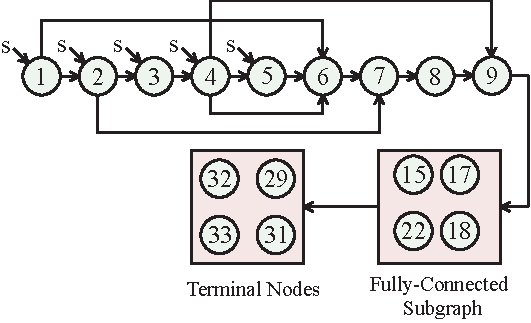
\includegraphics[width=0.6\linewidth]{figures/full2}
	\caption{The directed graph corresponding to a trojan.}
	\label{fig:full2}
\end{figure}
%%%%%%%%%%%%%%%%%%%%%%%%%%%%%
\subsection{Trojan Evaluation} \label{sec:techniqueEvaluation}
Due to the complexity of IC designs, hardware trojans are typically unique.
As a consequence, detection methods developed thus far have been developed to detect specific trojans.
The diversity in both trojans and detection methods makes it difficult to evaluate, compare, and organize them.
A means of evaluating hardware trojans and detection methods based on the eight attribute categories was proposed in~\cite{samerClassDetection}.
A trojan or detection method will possess some combination of attributes from each of the eight categories, and
each combination is assigned two numerical values.
The value $I$ is used to identify the combination, while the
value $C$ is used to denote the severity (for a trojan) or coverage (for a detection method) of the combination.
Tables of $I$ and $C$ values for the eight categories were presented in~\cite{samerDissertation}.
For example, the logic type category describes the circuit logic which activates the trojan.
Table~\ref{tbl:logicTypeTable} shows the possible attribute combinations for this category and the corresponding values of $I_L$ and $C_L$.
\begin{table}[h]
	\centering
	\caption{Logic Type Category Values}
	\label{tbl:logicTypeTable}
	\begin{tabular}{|c|c|c|}
		\hline
		Attributes & $I_L$ & $C_L$ \\ \hline
		Sequential (16) & 2 & 2 \\
		Combinational (17) & 1 & 1 \\
		Both (16 and 17)& 3 & 3 \\ \hline
	\end{tabular}
\end{table}

The $I$ and $C$ values from the category tables are arranged into identification and severity/coverage vectors, respectively.
For a trojan the vectors are denoted $I_T$ and $C_T$, and for a detection method they are denoted $I_D$ and $C_D$.
Thus, an identification vector is
\[
I = I_RI_AI_EI_LI_FI_CI_PI_O,
\]
where {$I_R,I_A,I_E,I_L,I_F,I_C,I_P,I_O$} are the
\{Insertion, Abstraction, Effect, Logic Type, Functionality, Activation, Physical Layout, Location\} category identification values, respectively, and
a severity/coverage vector is
\[
C = C_RC_AC_EC_LC_FC_CC_PC_O,
\]
where {$C_RC_AC_EC_LC_FC_CC_PC_O$} are the
\{Insertion, Abstraction, Effect, Logic Type, Functionality, Activation, Physical Layout, Location\} category strength values, respectively.

\begin{table}[h]
	\centering
	\caption{Identification and Severity Vectors for Two Hardware Trojans}
	\label{tbl:severityTable}
	\renewcommand{\arraystretch}{1.2}
	\begin{tabular}{|c|p{3mm}p{3mm}p{3mm}p{3mm}p{3mm}p{3mm}p{3mm}p{3.5mm}|p{3mm}p{3mm}p{3mm}p{3mm}p{3mm}p{3mm}p{3mm}p{3.5mm}|}
		\hline
		Technique & \multicolumn{8}{c|}{Parameters ($I_P$)} & \multicolumn{8}{c|}{Severity ($C_P$)} \\ \cline{2-17}
		& $I_R$ & $I_A$ & $I_E$ & $I_L$ & $I_F$ & $I_C$ & $I_P$ & $I_O$ & $C_R$ & $C_A$ & $C_E$ & $C_L$ & $C_F$ & $C_C$ & $C_P$ & $C_O$ \\ \hline
		Trojan A~\cite{samerAttribute} & 2 & 6 & 2 & 1 & 2 & 1 & 7 & 7 & \textbf{\textcolor{red}{2}} & 6 & 4 & 1 & 2 & 1 & 5 & 2 \\ \hline
		Trojan B~\cite{samerAttribute} & 3 & 3 & 1 & 2 & 1 & 2 & 8 & 1 & \textbf{\textcolor{red}{3}} & 3 & 2 & 2 & 1 & 3 & 6 & 1 \\ \hline
	\end{tabular}
\end{table}
\begin{table}[h]
	\centering
	\caption{Identification and Coverage Vectors for Two Hardware Trojan Detection Methods}
	\label{tbl:detectionTable}
	\renewcommand{\arraystretch}{1.2}
	\begin{tabular}{|c|p{3mm}p{3mm}p{3mm}p{3mm}p{3mm}p{3mm}p{3mm}p{3.5mm}|p{3mm}p{3mm}p{3mm}p{3mm}p{3mm}p{3mm}p{3mm}p{3.5mm}|}
		\hline
		Technique & \multicolumn{8}{c|}{Parameters ($I_P$)} & \multicolumn{8}{c|}{Coverage ($C_P$)} \\ \cline{2-17}
		& $I_R$ & $I_A$ & $I_E$ & $I_L$ & $I_F$ & $I_C$ & $I_P$ & $I_O$ & $C_R$ & $C_A$ & $C_E$ & $C_L$ & $C_F$ & $C_C$ & $C_P$ & $C_O$ \\ \hline
		\cite{method1} & 3 & 3 & B & 1 & 2 & 4 & 7 & V  & 3 & 3 & \textbf{\textcolor{red}{7}} & 1 & 2 & 3 & 5 & 5 \\ \hline
		\cite{method2} & 3 & 3 & 1 & 2 & 1 & 4 & 7 & V  & 3 & 3 & \textbf{\textcolor{red}{2}} & 3 & 1 & 3 & 5 & 5 \\ \hline
	\end{tabular}
\end{table}

Table~\ref{tbl:severityTable} provides a comparison of two hardware trojans.
Trojan A has a lower severity than Trojan B in the insertion category, denoted by $C_R$.
This indicates that Trojan B can be inserted in more stages of the manufacturing process than Trojan A.
Table~\ref{tbl:detectionTable} gives a comparison between two detection methods.
The method in \cite{method1} has a higher coverage in the effect category ($C_E$) than the method in \cite{method2},
indicating that it can detect more trojans based on their effects.
\section{Recent Work}
Hardware trojans are a new and exciting field of study.
As \acrshort{FPGA}s take a larger portion of the \acrfull{IC} market the need for security becomes greater.
With this, detection and analysis of trojans in \acrshort{FPGA}s has become a growing topic and has seen some development in recent years.
The majority of work focused on \acrshort{FPGA} trojans has employed either a means of reverse engineering, functional testing or 'side-channel' analysis.
The configuration \gls{Bitstream} contains all of the information one would want to know about what is happening on the device.
There has been little effort to directly analyze the \gls{Bitstream} because manufacturers are reluctant to provide intimate details of its format.
  
\subsection{\acrfull{CRC} Detection} \label{sec:crcDetection}
Because \acrshort{FPGA} design is done using a software language it is possible for designers to share component designs easily.
It is common for designers to employ 'third-party' \acrfull{IP}. 
This sharing of component design provides the opportunity for attackers to add trojans to commercial products by sharing trojan-containing \acrshort{IP}.
In 2013 researchers at Cairo University proposed a method of insulating externally sourced \acrshort{IP} with \acrfull{CRC} defense modules~\cite{crcDetection}.
According to the authors their method is capable of detecting leaked information with a 99.95\% accuracy.
This method employs a methodology referred to as 'built-in-self-test" (BIST) where additional hardware is added to the design.
The additional hardware performs run-time checking of circuit output.
In general, the BIST method is only capable of detecting modifications the designers have foreseen.
In this case, this method is only capable of detecting trojans that possess the attribute Information Leakage (13) from the taxonomy presented ins section~\ref{sec:topology}.
In addition the authors report considerable detriment to power consumption and performance.


\subsection{\acrfull{RO} Detection}
Researchers at the Technological Educational Institute of Western Greece and Industrial Systems Institute/RC “Athena” jointly proposed a method of using \acrfull{ROs} as a mechanism for detecting hardware trojans~\cite{ringOscillatorMethod}.
A \acrshort{RO} is a circuit composed of inverters formed into a loop.
Electric current looping through the \acrshort{RO} does so at an inherent frequency.
By configuring the circuit paths of the user's design into a \acrshort{RO} it is possible to create a 'signature'.
This signature is an expected frequency emitted from the desired design. 
The authors claim that modifications to the design will alter the frequency emitted by its circular configuration.
The experimental results showed that modifications did in-fact alter the frequency enough to reliably detect modifications.
This method can reliably detect hardware trojans but is incapable of providing any details regarding its effect.
Further, the stipulation that the desired design must be such that it forms an oscillating ring is impractical.
It is impossible to guarantee that all real-world designs can form an \acrshort{RO} whilst maintaining desired functionality and performance.
\subsection{The Multi-Faceted Approach}
Researchers from Iowa State University proposed a multi-faceted approach to trojan detection in \acrshort{FPGA}s~\cite{multiFacetedApproach}.
Their method composed of three approaches:
\begin{itemize}
	\item Functional Testing: A means of feeding test vectors and comparing the output to expected results.
	\item Power Analysis: Using an oscilloscope, the difference in power consumption between the desired design and the modified devices performing the same operations were recorded. Differences were used to discern the presence of a trojan.
	\item Bitfile Analysis: The authors attempted to employ a binary file analysis library named \textit{deBit}~\cite{bitStreamToNetlist} to reverse engineer a netlist from the \gls{Bitstream}.
\end{itemize}
The functional testing method attempted provided reasonable results. 
Test vectors used showed unexpected behavior; this provided only the information that a trojan was present.
The power analysis method again provided results of moderate quality.
With careful placement of the oscilloscope probes the authors were able to infer the physical location on the device where modifications occurred.
This provided no information however as to the relation between the modifications and the design.
Finally, the authors were able to only partially able to convert the \gls{Bitstream} to its netlist description.
Only descriptions of the primary logic circuit elements were achieved.
This could be used to discern some information regarding modifications discovered but is far from creating a complete description of a trojan.


\setlength{\unitlength}{\savedunitlength}